\chapter{Pre and Post processing work preparation}
\label{Pre and Post processing work preparation}


%----------------------------------------------------------------------------------------
%	SECTION 1
%----------------------------------------------------------------------------------------

\section{Abaqus software}

First, the purpose of this work is to compare the behavior of wood species with numerical analysis. That is why the preparation work begin by the modelling of MMCG specimen on Abaqus software. Abaqus allows to model a specimen, create a mesh, adapted to the geometry, initialize a crack, and obtain data from a virtual crack.

%----------------------------------------------------------------------------------------
%	SUBSECTION 1
%----------------------------------------------------------------------------------------

\subsection{Geometry and material creation}

The creation of the specimen follows the MMCG geometry specimen. It is explained in \parencite{Reference7} thesis. The different angles are taken into account and the four holes are created. The notch has a length of 25\si{\milli\meter}. 2D and 3D models were created. A 2.9\si{\milli\meter} line was put to continue the precrack and represent the cutter precrack done experimentally. 

Abaqus allows to create a material by adding his characteristics. In wood case as it is studied in this work, orthotropic characteristics must be inquired. Abaqus asks for a D matrix, defined as in \ref{eq:D matrix}
\begin{equation}
	\left[
	\begin{array}{rrrrrr}
		D_{1111} & D_{1122} & D_{1133} &
		0 & 0 & 0 \\
		D_{1122} &
		D_{2222} &
		D_{2233} &
		0 & 0 & 0 \\
		D_{1133} &
		D_{2233} &
		D_{3333} &
		0 & 0 & 0 \\
		0 & 0 & 0 &
		D_{1212} & 0 & 0 \\
		0 & 0 & 0 & 0 &
		D_{1313} & 0 \\
		0 & 0 & 0 & 0 & 0 &
		D_{2323} \\
	\end{array}
	\right]
	with : \\
	\\
	\left\{
	\begin{array}{lllll}
		D_{1111}=E_{1}(1-\nu_{23}\nu_{32})\gamma \\
		D_{2222}=E_{2}(1-\nu_{13}\nu_{31})\gamma \\
		D_{3333}=E_{3}(1-\nu_{12}\nu_{21})\gamma \\
		D_{1122}=E_{1}(\nu_{21}+\nu_{31}\nu_{23})\gamma \\	D_{1133}=E_{1}(\nu_{31}+\nu_{21}\nu_{32})\gamma	 \\	D_{2233}=E_{2}(\nu_{32}+\nu_{12}\nu_{31})\gamma \\	D_{1212}=G_{12} \\	D_{1313}=G_{13} \\	D_{2323}=G_{23} \\
	\end{array}
	\right.
	\label{eq:D matrix}
\end{equation}
It means that it is necessary before using ABAQUS to determine all these coefficients depending on the specie and the direction of the wood. These values for specimen at 12\% of MC which are the shearing $G_{ij}$ and longitudinal modulus $E_{i}$, the Poisson's coefficient $\nu_{ij}$ and $\gamma$ change for each species. After filling this D matrix it is possible to characterize the material of the specimen modelled. As an example, Okoume specie can be characterized by the values in \ref{eq:Okoume physicals values} which are confirmed by \parencite{Reference5}
\begin{equation}
	\left\{
	\begin{array}{llllllllllll}
		E_{1} = 9634 (MPa) \\
		E_{2} = 1090 (MPa)\\
		E_{3} = 522 (MPa) \\
		\nu_{12} = 0,369 \\
		\nu_{13} = 0,472 \\
		\nu_{23} = 0,705 \\
		\nu_{21} = \nu_{12}\dfrac{E_{2}}{E_{1}} = 0,042 \\
		\nu_{31} = \nu_{13}\dfrac{E_{3}}{E_{1}} = 0,026 \\
		\nu_{32} = \nu_{23}\dfrac{E_{3}}{E_{2}} = 0,338 \\
		G_{12} = 808 (MPa) \\
		G_{13} = 594 (MPa) \\
		G_{23} = 186 (MPa) \\
		\gamma = \dfrac{1}{1-\nu_{12}\nu_{21}-\nu_{13}\nu_{31}-\nu_{23}\nu_{32}-2\nu_{21}\nu_{32}\nu_{13}} = 1,387 \\
	\end{array}
	\right.
	\label{eq:Okoume physicals values}
\end{equation}
These values can evolve due to temperature and relative humidity. This is why, Guitard's model from \parencite{Reference2} are used. Indeed, by knowing the temperature, the relative humidity and the volume weight of a specimen, it is possible to obtain at least nine of the physicals values presented in \ref{eq:Okoume physicals values}. An important factor to obtain these parameters is also the wood type, hardwood or softwood. 

After the creation of the material by inputting the D matrix values. But also values as the density or the expansion coefficient linked to temperature. The material is assigned to the geometrical part.

%--------------------------------------------------------------%---------------
%	SUBSECTION 2
%----------------------------------------------------------------------------------------

\subsection{Load and boundary conditions}
Load and Boundary Condition (BC) must be also inquired. In 2 dimensions, the specimen was considered as blocked from one of the upper side. While the load is applied on the other upper side, even if the applied load is a surface one, localized in the hole as the BC. In 3 dimensions, load and BC are applied in the holes, so it must be closer to experimental conditions. The BC was considered as an embedding, even if in experimental conditions a displacement can occurs on the pin. So then, one dimension is considered as free. The magnitude was chosen at : 10\si{\kilo\newton}. The load type is considered as a "Surface Traction" and the added as a static load in a Global system x,y,z. The distribution is an uniform one and the direction, for this mode I Work, is perpendicular to the crack.

To provide the problem of a crack propagating from the hole, as it appears on some simulations, the area where the load is applied was considered as undeformed. The test expected is a dynamic one, working as an incremental process.

%----------------------------------------------------------------------------------------
%	SUBSECTION 3
%----------------------------------------------------------------------------------------

\subsection{Zone of Interest }
According to the tinny FPZ allows by MMCG geometry, the Zone of Interest must be well chosen. \parencite{Reference7} had already found ZOI shapes that allow the crack propagation study. By adapting the values to the dimensions of this work samples, a square of 2.8\si{\centi\meter} vertically and 5.6\si{\centi\meter} horizontally was created next to the precrack. As visible on \ref{fig:Abaqus_interface}
Then, three areas were also drawn as on \ref{fig:Abaqus_interface} and \ref{fig:Fig4}. The purpose of this ZOI and the 3 zones around the crack tip is to refine the analysis by creating a thinner mesh inside these areas. Indeed, the heel analysis is not relevant in a fracture mechanic problem as the crack study of this work. Whereas the evolution of this 3 areas allows to have a look to the Fracture Process Zone which go further with the time and the crack tip displacement.
One purpose is to obtain the stress concentration factor involves by the crack propagation on this ZOI.

%----------------------------------------------------------------------------------------
%	SUBSECTION 4
%----------------------------------------------------------------------------------------

\subsection{Mesh and link to finite element analysis}
Concerning the mesh, it is special on this geometry. But it will be focused on the crack and around it. The interest is to determine the displacement and the strain applied on the element of the mesh. That is why a ZOI was created \ref{fig:Fig16} and a thinner mesh was done in this area. Indeed, it is the interesting one, where the crack must develop. \parencite{Reference8} presented in the MMCG creation a mesh with element "tri" so triangular ones in many areas of the specimen. This mesh was really interesting because it is a radial one, with a center near the crack tip. It is localized at a constraint point. Moreover, the mesh in this area become a "quad" mesh, so rectangular elements or quadrilateral ones at least. In this work, "quad" elements were chosen.
\begin{figure}[h]
	\centering
	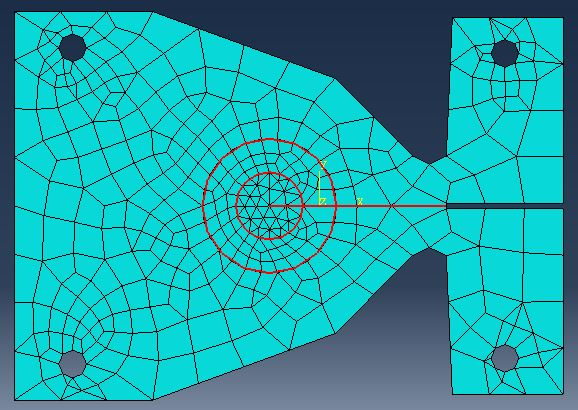
\includegraphics[scale=0.5]{Figures/Abaqus_Screenshot}
	\decoRule
	\caption[ABAQUS 2D specimen]{ABAQUS 2D Okoume specimen meshed with underlined ZOI and crack direction.}
	\label{fig:Fig16}
\end{figure}
Then, a step is created and also a job with the crack developement. This job allows to obtain a representation of the strain in each element of the mesh.
%----------------------------------------------------------------------------------------
%	SECTION 2
%----------------------------------------------------------------------------------------

\section{Python program}

%----------------------------------------------------------------------------------------
%	SUBSECTION 1
%----------------------------------------------------------------------------------------

\subsection{Initialization and input values}

The Python code developed is inspired from a previous one, done in MatLab by \parencite{Reference14} for DCB tests. MMCG specimen was created from DCB one, so it was logical to use this program with an adaptation to Python tools. 

The main purpose of this tool is to compute all the information given by DIC and obtain the energy release rate. To do that, it was reminded in \ref{eq:Energy release rate equation} that many parameters must be input. Some of them are constant and was measured before or after the test. It is the case for $a_{0}$ and "b" parameters, respectively, the initial crack length and the thickness of the specimen analyzed. It is defined in four big parts.

So a first program, allowing to combine all the constants by creating a structure as the one below, was done. It is called database and the following one is the example from the third Okoume specimen of the first experiment database:

\lstinputlisting[language=Python, firstline=1, lastline=9]{Codes/Database.py}

\begin{lstlisting}[language=Python]
	LX, H = 29.3, 1624  # mm / pixel
	if Job == 'e1o3':
	##########################################################################
	# pixel to mm magnification factor
	Test.mm2pixel = LX / H
	# Load conversion factor - testing machine
	Test.LoadConvFactor = 1000  # from kN to N
	# Displacement conversion factor - testing machine
	Test.DisplConvFactor = 2.0  # mm/V (gain = 20 mm)
	Test.thickness = 14 # unit  mm
	Test.a0 = 24.5 # unit  mm
\end{lstlisting}

\lstinputlisting[language=Python, firstline=11, lastline=19]{Codes/Database.py}

Thanks to this database file, open in the main code, many calls can be done and allow to synthesize the main code. Of course one database was created for each specimen and input in a single folder, due to the difference between values as the precrack length or the thickness of the specimen. Other values as the "Test.LoadConvFactor" will always be the same. Indeed, in this work, the load values, given by the MTS press are given in \si{\kilo\newton}, so a coefficient of 1000 must be added to obtain coherents results.

All the values from MatchID must be read and the displacement or load from the servohydraulic test machine have to been stored in Python variables. 

\begin{lstlisting}[language=Python]
	# determining the number of stages by inspecting MatchID processing files
	stages = glob.glob(os.path.join(cwd, 'DCB_002_*.tif.dat'))
	MatchID.stages = stages.__len__()
	print('Number of stages: ', str(MatchID.stages))
\end{lstlisting}

The first step is to store in a parameter, the number of stages by looking to the number of images captured by MatchID. As it is visible, variables are created, in a structure named MatchID. Here, the number of stages is stored in MatchID.stages variable. This MatchID structure is present in the database, because it is linked to each specimen. Indeed, the number of images changes from one test to another. So another part of the database is linked to MatchID settings and add information linked to this structure:  

\begin{lstlisting}[language=Python]
	# Summary of DIC Settings
	MatchID.CorrelationCoef = 'ZNSSD'
	MatchID.InterpolationOrder = 'Bicubic spline'
	MatchID.TransformationOrder = 'Affine'
	MatchID.Subset, MatchID.Step = 15, 13
	# Summary of Strain Settings
	MatchID.StrainWindow = 5
	MatchID.StrainConvention = 'GreenLagrange'
	MatchID.StrainInterpolation = 'Q4'
	# Area of Interest
	MatchID.Roi_PolyXi, MatchID.Roi_PolyYi = 52, 259
	MatchID.Roi_PolyXf, MatchID.Roi_PolyYf = 1587, 1119
\end{lstlisting}

It is possible to use, thanks to this part, the type of subset used, the steps, the strain window and interpolation, previously chosen, looking on the best parameters on MatchID curves. Then, the displacements and load of every stages must be stored to. In order to do it, an iterative loop is created :

\begin{lstlisting}[language=Python]
	# U displacement
	UX = np.zeros((MatchID.SubsetsY, MatchID.SubsetsX, MatchID.stages))
	tic()
	for i in np.arange(0, MatchID.stages, 1):
	readstr = #Name of the test
	print('reading : ',readstr)
	pathdados = os.path.join(cwd,'u',readstr)
	aux = np.genfromtxt(pathdados, skip_header=0, delimiter=';')
	UX[:, :, i] = aux[:, :-1]*Test.mm2pixel # unit: mm
	print(f'{toc():.1f} seg')
\end{lstlisting}

This loop stores the displacement on U direction, but another similar one do the same on V direction. Ux is a Matrix filled by the reading of MatchID.subset file and the number of stages. Then it is multiply by the convector factor from pixel to \si{\milli\meter}. 

%----------------------------------------------------------------------------------------
%	SUBSECTION 3
%----------------------------------------------------------------------------------------

\subsection{Determination of the CTOD} 

After computing all the data from the database, a second part is computed. It is linked to the Crack Tip Opening Displacement (CTOD). Indeed, this factor has impact on the cohesive law. MatchID is a great tool which does some work for the user. That is why, some of the information from the software program were put in the Database, as in the next code with the ZOI dimensions: 
\begin{lstlisting}[language=Python]
	# Allied Manta G-505B
	H, V  = 2448, 2050 # unit: pixels
	# 'TC2336' telecentric lens
	LX, LY = 34.98, 29.18 # unit: mm
\end{lstlisting}

Then, two matrix are created. There are first, declared and made of zeros :

\begin{lstlisting}[language=Python]
	CTODI  = np.zeros((ud_lim, 3, MatchID.stages))
	# Vup, Vdown, ||Vup-Vdown||
	CTODII = np.zeros((ud_lim, 3, MatchID.stages))
\end{lstlisting}

As shown in the code, the dimensions of the matrix take in account the number of stages, so the number of images. Indeed, the interest of the CTOD is to be followed at each stage. 

Then, a loop is created, allowing to put information into others vectors

\begin{lstlisting}[language=Python]
	for J in np.arange(0, MatchID.stages, 1):
	# mode I:
	uYtemp = np.copy(UY[:, :, J])
	CTODI[:, 0, J] = np.flipud(uYtemp[a0.Y - ud_lim: a0.Y, a0.X])
	CTODI[:, 1, J] = uYtemp[a0.Y: a0.Y + ud_lim, a0.X]
	CTODI[:, 2, J] = np.abs(CTODI[:, 1, J] - CTODI[:, 0, J])
\end{lstlisting}

Another one is also created to compared to mode II values. In the current case, the mode II can be approximate around zero, because it is a mode I test. Then all the values are obtained, for each COD pair until $ud_lim$ which is in this case equal to 10. By looking to this different curves, the chosen COD pair is chosen and a curve is plot looking to the values for this parameter chosen by the user. 

\begin{figure}[h]
	\centering
	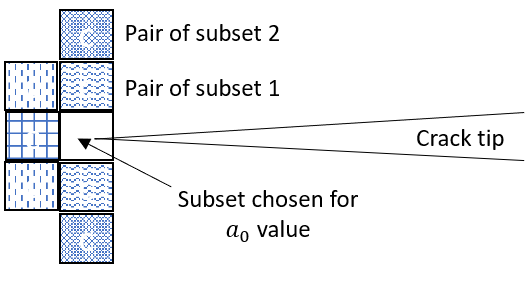
\includegraphics[scale=0.7]{Figures/Subset_choice}
	\decoRule
	\caption[Subset choice and pair of subset around]{Pair of subset around the $a_{0}$ subset chosen}
	\label{fig:subest_chosen}
\end{figure}

Finally, the way to obtain CTOD, need also a well $a_{0}$ choice. Indeed, the chosen subset as presented on \ref{fig:subest_chosen}, will be determinant. Considering the image as a matrix composed of subset, the chosen subset as a position given by his m row and n column. To determinate the opening, it is necessary to have a look on the subsets in the same n column but at a different line. Indeed, the chosen subset will be the first one affected by the crack, that means, that information on the subset will not have importance anymore. While, looking to subset up and down allow to follow the displacement of the crack tip and measure it. The fact is to determine which pair of subsets is the best. The ones at the row n-1 and n+1, but maybe these ones will be on the crack at a given stage, and will lose all the necessary information. That is why, an important choice must be done. Here, COD pair was fixed equal to two. So the subset displacement analysed is the one of the pair of subset 2 on \ref{fig:subest_chosen}. Finally, by looking to these displacements, it is possible to obtain the value of the crack opening at each stages.

%----------------------------------------------------------------------------------------
%	SUBSECTION 4
%----------------------------------------------------------------------------------------

\subsection{Crack length analysis}

The third part of the code has the purpose to determine a(t), so the crack length evolution. This evolution can be compared to the time or the servohydraulic test machine displacement and also the load applied on the specimen. The first step is again to define everything. The displacement are stored again, the Zone Of Interest (ZOI) is defined by suppressing the value out of this ZOI.
This a(t) parameter is the most difficult to obtain, indeed tools as MatchID cannot help the user to obtain the result stage by stage. The value of a(t) will be equal to $a_{0}$ fixed by the user and add to a $\Delta a$ which is the value of the crack length, evolving in time due to the applied force.

\begin{lstlisting}[language=Python]
	displ_x = UX[:,:,J]
	displ_y = UY[:,:,J]
	# resize RoI containing the crack growth process
	if roi == 'crop':
	displ_x = displ_x[Y_i:Y_f,X_i:X_f]
	displ_y = displ_y[Y_i:Y_f,X_i:X_f]
	
	# find the dimensions of the matrix
	m = displ_x.shape[0] #  y - row
	n = displ_x.shape[1] # x - column
	# find the matrix with the displacements
	displ = (displ_x**2 + displ_y**2)**0.5
	# preallocation: zeros
	n_zeros = np.zeros((m, 1))
	m_zeros = np.zeros((1, n+1))
\end{lstlisting}

After defining all the parameters, the displacement of the crack tip is observed thanks to some calculus on the subsets. 

\begin{lstlisting}[language=Python]
	displ_A = np.vstack((np.hstack((displ,n_zeros)), m_zeros))/4
	# divided by 4 because sum: displ_A+displ_B+displ_C+displ_D
	displ_B = np.vstack((np.hstack((n_zeros,displ)), m_zeros))/4
	displ_C = np.vstack((m_zeros, (np.hstack((displ, n_zeros)))))/4
	displ_D = np.vstack((m_zeros, (np.hstack((n_zeros, displ)))))/4
	# auxiliar matrix 2 edges; 4 within the matrix 'matr_transf'
	matr_transf = np.ones((m+1, n+1))
	matr_transf[:, 0] = 2
	matr_transf[:, -1] = 2
	matr_transf[0, :] = 2
	matr_transf[-1, :] = 2
	matr_transf[0, 0] = 4
	matr_transf[0, -1] = 4
	matr_transf[-1, 0] = 4
	matr_transf[-1, -1] = 4
	grid_values = (displ_A + displ_B + displ_C + displ_D)*matr_transf
	# displacements of each corner on the facet
	displ_A = grid_values[0:-1, 0:-1]
	displ_B = grid_values[0:-1, 1:]
	displ_C = grid_values[1:, 0:-1]
	displ_D = grid_values[1:, 1:]
	# oblique distance between facet centroids
	displ_CA = np.abs(displ_C-displ_A)
	displ_DB = np.abs(displ_D-displ_B)
	# auxiliar function for the crack tip location criterion
	K = np.maximum(displ_CA, displ_DB)
	avgK = np.nanmean(K) #mean ignoring nan values.
	stdK = np.nanstd(K)
	maxK = np.nanmax(K)
	if maxK < avgK + inb*stdK:
	J = J + 1
	else:
	JJ = 0
\end{lstlisting}

Here, all the matrix, composed of the subsets from the Zone of Interest are changed by the different steps shown overhead. All the subsets are considered four by four and operations are done on them. The displacement from one compared to it neighbor are computed. Then average and maximum values are obtained for each subset of the ZOI and put into K matrix. By using the $a_{0}$ data and looking to the alpha parameter, permitting to compute the best shape of a(t), having the more precise values but numerous ones also, a(t) is obtained with a similar method. It must be noticed, that to determinate a(t) parameter, $\alpha$ parameter is needed. This one is used on matrix as the M matrix. Indeed, M matrix represents, for a given stage, the crack length by having bigger value in the crack area as shown on \ref{fig:Fig11} : 

\begin{figure}[h]
	\centering
	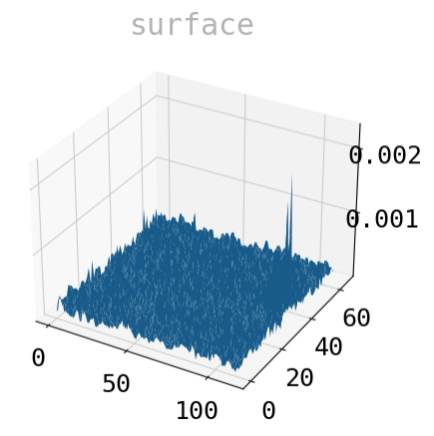
\includegraphics[scale=0.5]{Figures/M_matrix}
	\decoRule
	\caption[M matrix]{M matrix, obtained by running python code}
	\label{fig:Fig11}
\end{figure}

As it is visible, if the user is looking too close, the noise of the values will avoid a good analyze, but by looking too high on the matrix, the crack length value will not be accurate. To move and have a precise idea of the way the user can watch the M matrix, it is important to use $\alpha$. Alpha parameter is like a cutting tool which allows to be as close as the noise without troubles.
To approximate the $\alpha$ value, a correlation factor is searched by least square regression method. The objective it to have the best linear part. A plot is created to show which stage is the most appropriate as on \ref{fig:Fig12}.

\begin{lstlisting}[language=Python]
	### 2 criterion for checking stage
	####
	inb = 3
	# standard deviation * inb (to be checked by user)
	# inb = 1: 68.3 %
	# inb = 2: 95.4 %
	# inb = 3: 99.7 %
\end{lstlisting}

It is possible to adapt the alpha parameter precision by choosing a different "inb" as presented in the code overhead. Indeed, the correlation factor change depending on this criterion. The chosen stage is the one, before the beginning of the crack propagation, but the nearest to the expansion of a(t) length.

\begin{figure}[h]
	\centering
	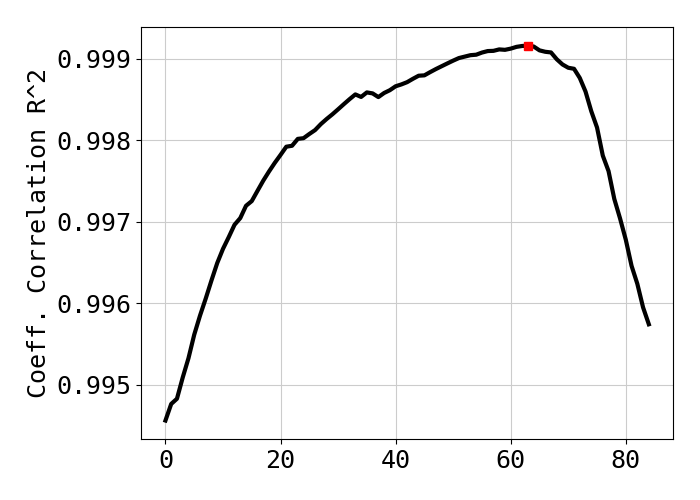
\includegraphics[scale=0.3]{Figures/Correlation_factor}
	\decoRule
	\caption[R correlation factor]{R correlation factor allowing to know which load and displacement is linked to crack beginning.}
	\label{fig:Fig12}
\end{figure}

This method was the one used by \parencite{Reference14} on MatLab, and have already proved obtention of good results.

%%----------------------------------------------------------------------------------------
%%	SUBSECTION 5
%%----------------------------------------------------------------------------------------
\subsection{Compliance and Energy values}

The last part of the code consists in using all the calculated parameters, in order to obtain the energy release rate. It is done by computing the G formula as presented below.

\begin{equation}
	G_{c}= \frac{F_{c}^2}{2b} (\frac{\Delta C}{\Delta a})_{d} 	
	\label{eq:Energy release rate equation}
\end{equation}

This equation, already given, is written on Python as :

\begin{lstlisting}[language=Python]
	a_t = crackL_J_mm[:,chos_alp]
	
	C = MatchID.displ/MatchID.load
	
	# P**2/2/B* dC / da
	ALP = (MatchID.load**2)/(2*Test.thickness)
	
	# C = MatchID.displ/MatchID.load
	
	# BET = C/a_t #changing the value of alpha from the crack length will change G values
	#
	G = ALP*BET
	# G = np.dot(ALP,BET)
\end{lstlisting}

In this case, the formula used, is the simplest one, which allow to easily obtain C by dividing the displacement from servohydraulic test machine by the load. These values are stored in MatchID variable, allowing to synthesize all the data in one per image (stage). An average are done on the seven values between two images. This fact can also involve a little mistake.
Therefore, as explained in "alpha" and "a(t) determination" sections, the crack length depends on alpha parameter. So some curves are plotted depending on "a(t)" matrix changes according to the alpha. The best R-curves must be determined for the most precise crack length. So it is necessary to find a great alpha parameter to have these final values without huge mistake.

\begin{lstlisting}[language=Python]
	# write array results on a csv file:
	RES = np.array([MatchID.displ[:], MatchID.load[:], C[:], COD.wI[:], a_t[:], G[:]])
	RES = np.transpose(RES)
\end{lstlisting}

At least, values as the displacement, the load, the compliance, the CTOD, the crack length and the energy release rate, are stored into a matrix and then exported to .csv files. It allows saving data, but also to compute everything in Excel in addition to python processing tool.

Many improvements are made on the Python code, even after this work ended. Indeed, it appears that the crack length can be better compute, in order to avoid some strange shapes of R-curves. But using the same tool for all specimens computation, even if mistakes exist, it is possible to compare data.


%\section{Python program}
%
%%----------------------------------------------------------------------------------------
%%	SUBSECTION 1
%%----------------------------------------------------------------------------------------
%
%\subsection{Initialization and input values}
%
%The Python code developed is inspired from a previous one, done in MatLab by \parencite{Reference14} for DCB tests. MMCG specimen was created from DCB one, so it was logical to use this program with an adaptation to Python tools. A first program, allows to combine all the constants by creating a structure as :
%
%\begin{customFrame}
%	# pixel to mm magnification factor
%	Test.mm2pixel = LX / H
%	# Load conversion factor - testing machine
%	Test.LoadConvFactor = 50  # N/V (gain = 500 N)
%	# Displacement conversion factor - testing machine
%	Test.DisplConvFactor = 2.0  # mm/V (gain = 20 mm)
%	Test.thickness = 12.5 # unit  mm
%	Test.a0 = 20 # unit  mm
%	###################################################
%	# Summary of DIC Settings
%	MatchID.CorrelationCoef = 'ZNSSD'
%	MatchID.InterpolationOrder = 'Bicubic spline'
%	MatchID.TransformationOrder = 'Affine'
%	MatchID.Subset, MatchID.Step = 15, 13
%	# Summary of Strain Settings
%	MatchID.StrainWindow = 5
%	MatchID.StrainConvention = 'GreenLagrange'
%	MatchID.StrainInterpolation = 'Q4'
%	# Area of Interest
%	MatchID.Roi_PolyXi, MatchID.Roi_PolyYi = 52, 259
%	MatchID.Roi_PolyXf, MatchID.Roi_PolyYf = 1587, 1119
%	###################################################
%	# Selecting subset directly from MatdhID
%	a0.imgH, a0.imgV = 1529, 669
%	# Selecting pair
%	COD.cod_pair = 2
%	
%\end{customFrame}
%
%Thanks to this database file, open in the main code file, many calls can be done and allow to synthesize the main code. Of course one database was created for each specimen, due to the difference between values as the precrack length or the thickness of the specimen. Other values as the "Test.LoadConvFactor" will always be the same. Indeed, in this work, the load values, given by MTS servohydraulic test machine are given in \si{\kilo\newton}, so a coefficient of 1000 must be added to obtain coherent results.
%
%This main code is composed of several parts. First, after defining modules, path and opening all the necessary files as displacement csv file or strain one, it is important to read all the images from a single test. Indeed, it allows to know the number of stages (images) which must be run to obtain the entire test. Each stage gives a displacement of pixels, so un displacement of subsets, allowing to follow the crack length and the crack opening. It is important to note that MatchID allows to focus on a Zone of Interest (ZOI) in order to limit the amount of subsets read. According to \parencite{Reference7} dimensions of this ZOI are given for biggest specimens. By using equivalent dimensions, the ZOI adapted to this thesis is around 5,6\si{\centi\meter} length from the upper holes of the specimen and 2,8\si{\centi\meter} of width.
%
%Then, by using the displacement depending on the axis, x and y, two folders are read, one with x displacements, the other with y displacements. In each folder, one test is composed of a number of files equal to the number of stages. It gives information about pixel movement. By reading these two folders, a first graphic is created, giving a representation of the specimen, with the subsets presented and the subset chosen to be the $a_{0}$ one (closer to the crack tip).
%
%%----------------------------------------------------------------------------------------
%%	SUBSECTION 2
%%----------------------------------------------------------------------------------------
%
%\subsection{Alpha parameter}
%
%To begin with, it is important to determinate a parameter, that we had called $\alpha$. This one is used on matrix as the M matrix. Indeed, M matrix represents, for a given stage, the crack length by having bigger value in the crack area as shown on \ref{fig:Fig11} :
%
%\begin{figure}[h]
%	\centering
%	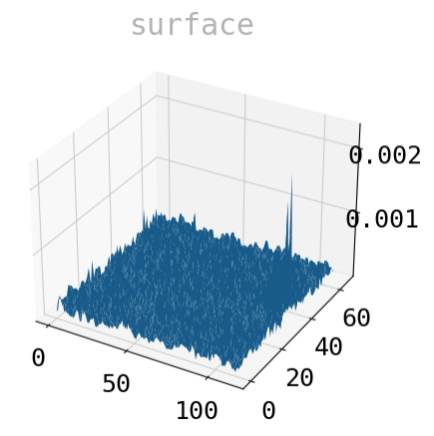
\includegraphics[scale=0.5]{Figures/M_matrix}
%	\decoRule
%	\caption[M matrix]{M matrix, obtained by running python code}
%	\label{fig:Fig11}
%\end{figure}
%As it is visible, if the user is looking too close, the noise of the values will avoid a good analyze, but by looking too high on the matrix, the crack length value will not be accurate. To move and have a precise idea of the way the user can watch the M matrix, it is important to use $\alpha$. Alpha parameter is like a cutting tool which allow to be as close as the noise without troubles.
%To approximate the $\alpha$ value, a correlation factor is searched by least square regression method. The objective it to have the best linear part.
%\begin{customFrame}
%	#### alpha evaluation
%	### Selecting stage for investigating alpha
%	####
%	# least-squares linear regression
%	porder = 1
%	xx = Test.disp # displacement (mm)
%	yy = Test.load # load (N)
%	# Data point in the linear least-squares regression
%	limsup = int(0.75*np.argwhere(max(yy)==yy)[-1])
%	# number of maximum data points for LSR
%	liminf = int(np.round((1/3)*limsup))# number of minimum data points for LSR
%	
%	xx, yy = xx[0:limsup], yy[0:limsup]
%	Rtot = np.zeros((limsup-liminf,1))
%	C_M = np.zeros((limsup-liminf,1))
%	for j in np.arange(0,limsup-liminf,1):
%	limt_sup = liminf + j
%	xfit, yfit = xx[0:limt_sup], yy[0:limt_sup]
%	p  = np.polyfit(xfit, yfit, porder)
%	C_M[j] = 1/p[0]
%	dev = yfit - np.mean(yfit) # deviations - measure of spread
%	SST = np.sum(dev**2) # total variation to be accounted for
%	resid = yfit - np.polyval(p, xfit) # residuals - measure of mismatch
%	SSE = np.sum(resid**2) # variation NOT accounted for
%	Rtot[j] = 1 - SSE/SST #  variation NOT accounted for
%	
%	# position for the best fitting point parameters
%	jmax = np.max(np.argwhere(np.max(Rtot)==Rtot))
%	J = int(liminf + jmax)
%	
%	### 2 criterion for checking stage
%	####
%	inb = 3
%	# standard deviation * inb (to be checked by user)
%	# inb = 1: 68.3 %
%	# inb = 2: 95.4 %
%	# inb = 3: 99.7 %
%	JJ = 1
%	while JJ == 1:
%	\end{customFrame}
%	
%	\begin{figure}[h]
%	\centering
%	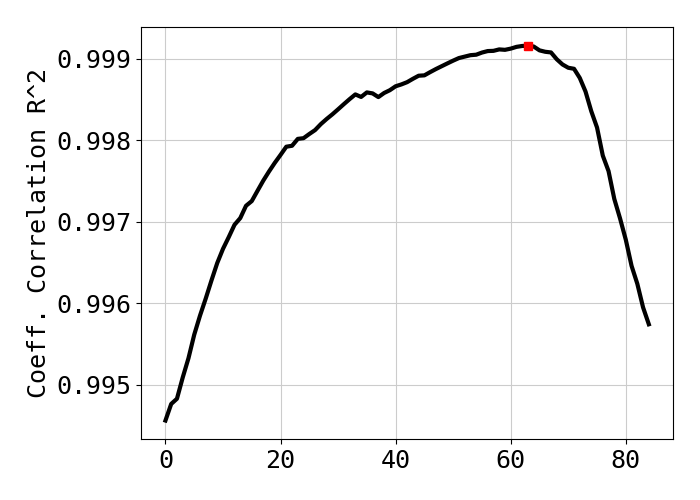
\includegraphics[scale=0.3]{Figures/Correlation_factor}
%	\decoRule
%	\caption[R correlation factor]{R correlation factor allowing to know which load and disalcement is linked to crack beggining.}
%	\label{fig:Fig12}
%	\end{figure}
%	
%The red dot shown on \ref{fig:Fig12}, is linked to another plot,
%	
%Then a matrix representing the subsets in the Area of Interest will be created. First this matrix is composed of zero. Then, the four corners of the matrix will be used to proceed several operations on the matrix. The external lines and columns will take a value of 2 and the corners a value of 4. The distance between opposite corners is calculated and their displacements are compared. Calling K, the maximal displacement of the two corners, average K and maximum one between all the steps are compared. Again, every subset is treated and are still zero when the material is undamaged. It becomes -1 in a region where the material is damaged, and no information are treatable. And it becomes 1 where a discontinuity appears but the wood is not completely damaged like the crack tip. So, by following the farthest 1 value in the matrix, it is possible to know the last subset where the crack tip is localized. Thanks to this distance, some conversions are necessary, from subset to pixel first, and then from pixel to millimeters. Finally, the crack length is determined depending on stages so it could be linked to load or displacement, and thanks to the previous work, to CTOD. The compliance is calculated by dividing the displacement by the load. G is the last variable calculated, with all the previous variables determined, as CTOD presented below and a(t). The last plot is the R-curve representing the Energy release and the crack length.
%%----------------------------------------------------------------------------------------
%%	SUBSECTION 3
%%----------------------------------------------------------------------------------------
%
%\subsection{Determination of the CTOD}
%
%Another partof the code has the purpose to calculate the Crack Tip Opening Displacement (CTOD). MatchID is a great tool which does some work for the user. That is why, by using “wI aramis2D.csv” CTOD is almost find, depending on the time and the load applied. It is important to understand how it works.
%
%First, a part of the work is to define the zone of interest (ZOI), the one where the crack must develop. It is done on MatchID, but also on Python by using the number of the subset defined by Match ID. Then, when a subset is out of this region, it will be considered as equal to zero. Then, the subsets which are placed into the crack, or somewhere where there is a default or missing information as into the crack, the substep will be defined with a value equale to -1. Then, for all the substep around the crack, which have a real interest in the study, they will take the value equal to 1. By using this matrix of substep, now, composed of -1, 0, 1 value, it is possible to plot the entire matrix into grey nuances, and have a look at the crack development, by adding matrix, given by different stages.
%
%\begin{customFrame}
%ud_lim = 10
%# Uup, Udown, ||Uup-Udown||
%CTODI  = np.zeros((ud_lim, 3, MatchID.stages))
%
%for J in np.arange(0, MatchID.stages, 1):
%# mode I:
%uYtemp = np.copy(UY[:, :, J])
%CTODI[:, 0, J] = np.flipud(uYtemp[a0.Y - ud_lim: a0.Y, a0.X])
%CTODI[:, 1, J] = uYtemp[a0.Y: a0.Y + ud_lim, a0.X]
%CTODI[:, 2, J] = np.abs(CTODI[:, 1, J] - CTODI[:, 0, J])
%COD.wI = CTODI[COD.cod_pair, 2, :]
%\end{customFrame}
%
%\begin{figure}[h]
%	\centering
%	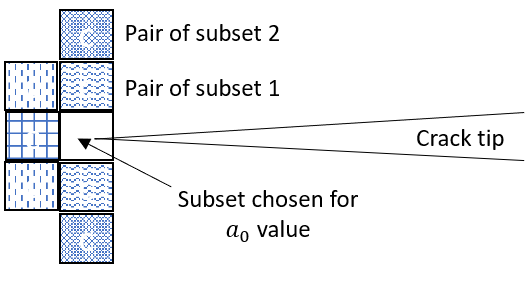
\includegraphics[scale=0.7]{Figures/Subset_choice}
%	\decoRule
%	\caption[Subset choice and pair of subset around]{Pair of subset around the $a_{0}$ subest chosen}
%	\label{fig:subest_chosen}
%\end{figure}
%
%To obtain CTOD, it is important to be careful to $a_{0}$ choice. Indeed, the chosen subset as presented on \ref{fig:subest_chosen}, will be determinant. Considering the image as a matrix composed of subset, the chosen subset as a position given by his m row and n column. To determinate the opening, it is necessary to have a look on the subsets in the same n column but at a different line. Indeed, the chosen subset will be the first one affected by the crack, that means, that information on the subset will not have importance anymore. While, looking to subset up and down allow to follow the displacement of the crack tip and measure it. The fact is to determine which pair of subsets is the best. The ones at the row n-1 and n+1, but maybe these ones will be on the crack at a given stage and will lose all the necessary information. That is why, an important choice must be done. Here COD pair was fixed equal to two. So the subset displacement analyzed is the one of the pair of subset 2 on \ref{fig:subest_chosen}. Finally, by looking to these displacements, it is possible to obtain the value of the crack opening at each stages.
%
%%----------------------------------------------------------------------------------------
%%	SUBSECTION 4
%%----------------------------------------------------------------------------------------
%
%\subsection{Crack length analysis}
%
%At least, an important step in this code is the determination of $a_{DIC}$. This parameter is the crack length, which evolves with time during all the experiment. This factor is the most difficult to obtain, indeed tools as MatchID cannot help the user to obtain the result stage by stage. The value of a(t) will be equal to $a_{0}$ fixed by the user and additional to a $\Delta a$ which is the value of the crack length, evolving in time due to the applied force.
%
%\begin{customFrame}
%roi = 'crop' # 'all'; 'crop'
%i, incr = 1, 1
%# incr : is used to step over stages if required (default = 1: all stages)
%Y_i, Y_f = 0, UY.shape[0]
%X_i, X_f = 0, a0.X
%\end{customFrame}
%
%\begin{customFrame}
%	# estimation of crack tip length
%	tipstep = np.zeros((alphaint.shape[0],1)) # unit: substep
%	tipmm = np.zeros((alphaint.shape[0],1)) # unit: mm
%	
%	for kk in np.arange(0,alphaint.shape[0],1):
%	alpha = alphaint[kk]
%	# Criterion for crack tip location
%	Kt = np.zeros(K.shape)
%	Kt[np.isnan(K)] = -1
%	Kt[K>=alpha*avgK] = 1
%	Ktemp = Kt
%	# n1 which must be relative to 'a0'
%	ind = np.argwhere(Ktemp==1)
%	row, col = ind[:,0], ind[:,1]
%	if len(col) == 0:
%	tipstep[kk] = 0
%	else:
%	tipstep[kk] = a0.X - np.min(col) # X component
%	# pixel>mm: [macro-pixel*(pixel/macro-pixel)*(mm/pixel)
%	tipmm[kk] = np.abs(tipstep[kk]*MatchID.mm2step - MatchID.mm2step)
%	
%	# for selected  alpha parameters you compute crack length
%	# crack length however should be ZERO at the beginning (no crack propagation)
%	ind = np.where(np.abs(tipmm - np.min(tipmm)) == 0)
%	alpha_alphasel = alphaint[ind[0][0]]
%	\end{customFrame}
%A final part of the code allows to obtain a(t) depending on alpha  as it is done on \parencite{Reference14} article. It is done by a focus on the ZOI and the number of subsets composing it. Thanks to the matrix composed by every subsets, the displacement field can be observed. It is obtained by computing the distance between the center of a subset and it displacement from one image to the next one as shown in the literature review. To simplify the code, it is not done on every subset but only on the four corners. By computing the distance between the opposite corners, the maximum x-displacement and an y-displacement are input in a last matrix. 
%
%%----------------------------------------------------------------------------------------
%%	SUBSECTION 5
%%----------------------------------------------------------------------------------------
%
%\subsection{Compliance and Energy values}
%
%As said in alpha parameter section, The last step is to compute the Compliance and then the Energy release rate. Indeed, all the necessary parameters are present in the Python variables. So by computing the formula \ref{eq:Energy release rate equation} the different matrix composed of all the values depending on the stage are used to obtain first a compliance matrix with same dimensions of the CTOD and the dispacement of the servohydraulic test machine matrix created.
%
%As presented in this part of the code, after calculating G, some plots are created. But as explained in "alpha" and "a determination" sections, the crack length depends on alpha parameter. So some curves are ploted depending on "a" matrix changing according to the alpha.And the best R-curves must be determined for the best crack length. It is necessary to find the best alpha parameter to have these final values.
%
%Finaly, 
%----------------------------------------------------------------------------------------
%	SECTION 3
%----------------------------------------------------------------------------------------

\section{Experimental devices}


%----------------------------------------------------------------------------------------
%	SUBSECTION 1
%----------------------------------------------------------------------------------------

\subsection{Arcan model and Final Grips}

MMCG specimens were created to be tested in every fracture mechanics modes. But as presented in the literature review, to be tested in every mode, the load must be applied in different direction. That is why the first grips designed were Arcan ones. Indeed, by changing the way of fixation between each part, it is possible to applied load with 10\textdegree of difference between each fixation point. Thanks to Catia software, the same prototype as the one used by \parencite{Reference7} and \parencite{Reference6} was created as on \ref{fig:Arcan}.

\begin{figure}[h]
	\centering
	\begin{subfigure}{0.48\linewidth}
			\centering
			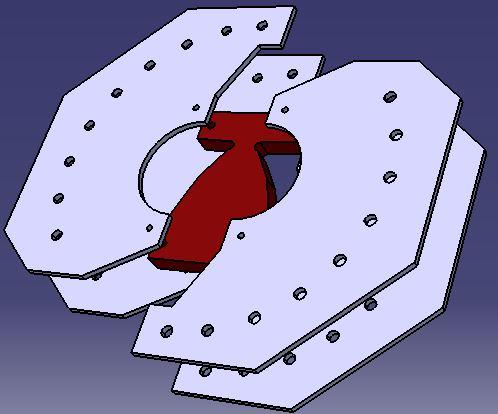
\includegraphics[scale=0.5]{Figures/Result}
			\decoRule
			\caption[Arcan grips]{Arcan design on Catia software}
			\label{fig:Arcan}
	\end{subfigure}
	\hfill
	\begin{subfigure}{0.48\linewidth}
		\centering
		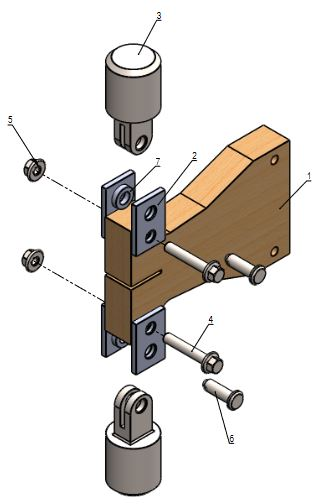
\includegraphics[scale=0.4]{Figures/Grips_model}
		\decoRule
		\caption[Grips modelled]{Mode I grips model composed of 1 : the wood part, 2 : plates 2ISO 4162 - M5 x 30 x 16-C, 3 : Screw part 34 CrNiMo 6, 4 : screw fixing spcimen, 5 : nut, 6 : pin, 7 : washers}
		\label{fig:Grips_model}
	\end{subfigure}
	\hfill
	\begin{subfigure}{0.48\linewidth}
		\includegraphics[scale=0.04]{Figures/Grips}
		\decoRule
		\caption[Grips]{Grips used to connect the Hydraulic press to the spcimen.}
		\label{Grips}
	\end{subfigure}
	\caption{Grips components evolution}
	\label{Grips components evolution}
\end{figure}

In addition with screw and nut placed in the heel holes and, in the case of this work, in the 90\textdegree Arcan system holes, mode I experiments could be done. But this work is focusing on mode I and do not need this heavy plates of steel or PVC in the case of \parencite{Reference8} works.

So the final grips are presented in \ref{fig:Grips_model} and \ref{Grips}. These ones, simpler than ARCAN system, only allow to do mode I experiments. They were designed especially for MMCG dimensions and manufactured near Caparica campus. The system is composed of a main piece which can be added in the mechanical press by screwing it inside. Then, a pin allows to place two connectors from each side of the MMCG specimen. It was induced that the connectors, if they were well tight, could play washers role. Indeed, \parencite{Reference7} as shown the importance of glued washers to provide a crack from the holes. Finally, another pin goes through the connectors and the specimen holes. Experiments have shown that washers are still essential, so they were added as it is visible on \ref{fig:Grips_model} second caption.

It must be noted that, due to the pandemic situation, the grips have taken time to be designed and received. Due to this delay, the experiments have begun only in June.

%----------------------------------------------------------------------------------------
%	SUBSECTION 2
%----------------------------------------------------------------------------------------

\subsection{Servohydraulic test machine used}


To determine the load speed, the frequency of the camera recording and others experimental parameters, it was important to read previous works on the subject and determine which engines will be used to proceed the experiments. The hydraulic press used to pull on each side of the specimen is shown on \ref{fig:HydrauPress}, it is the MTS servohydraulic test machine, model 661.21B-03 allowing a maximal applied load of 100 \si{\kilo\newton}

\begin{figure}[th]
	\centering
	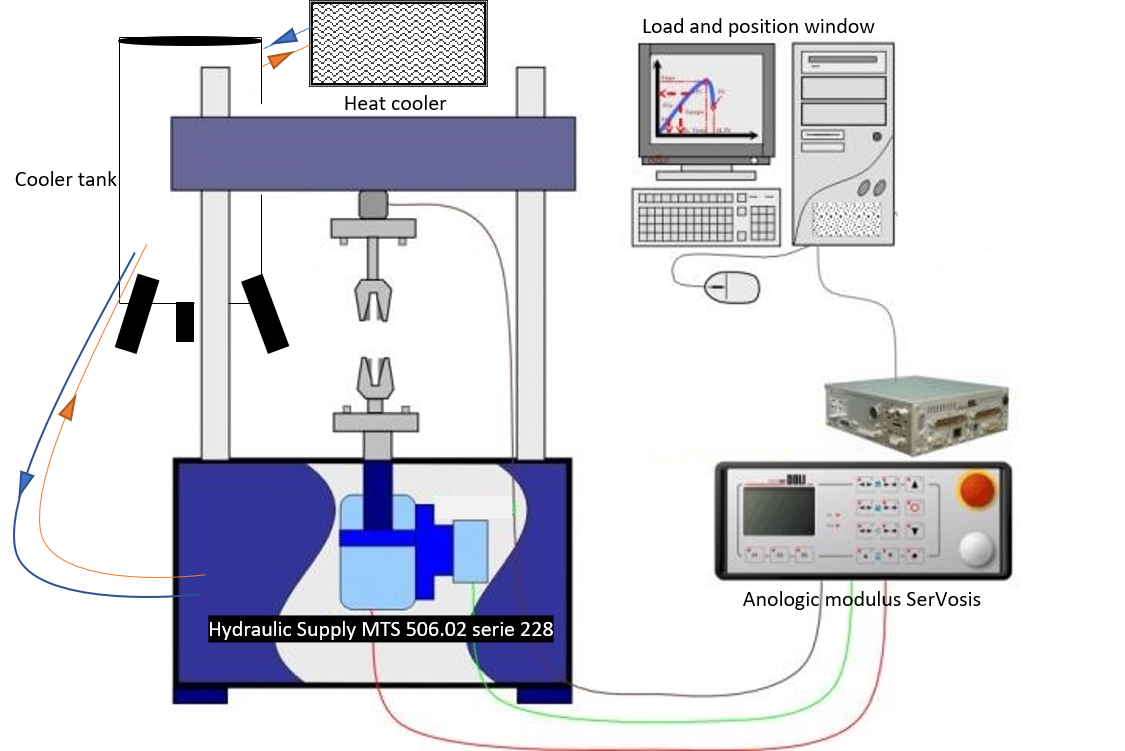
\includegraphics[width=\textwidth]{Figures/Hydraulic_Press2}
	\decoRule
	\caption[Hydraulic Press fonctionnement]{Hydraulic Press components allowing it use}
	\label{fig:HydrauPress}
\end{figure}
	
\parencite{Reference17} works allow to find how the load must be applied. Indeed, it gives an approximation of loads values or displacement speed. The load speed recommended is about 0,1\si{\milli\meter\per\minute} according to these texts. \parencite{Reference7} used the same loading speed around 5\si{\milli\meter\per\minute}. The records are made at a frequency of 5Hz, so 5 images per second, according to \parencite{Reference17} or \parencite{Reference16}.
\parencite{Reference7} works helps to specify this type of parameters on MMCG samples. It is obvious that there are many similitude with DCB works. Indeed, MMCG geometry is an adaptation of DCB and CTS ones, that explain why many parameters are the same. It must be reminded that this press is also chosen because of this possibilities to load specimens by a constant time displacement. Indeed, it was explained that this work will use complacency method to compare the results.


This MTS servohydraulic test machine works in addition with a cooler fluid. Indeed, in a room close to the testing one, a tank full of fluid mixed to water and a cooler system send this fluid mix to the press as visible on \ref{fig:HydrauPress}. Then a hydraulic supply from MTS company send this liquid to the press itself. It is  the model 506.02 serie 22 coupled with the Vickers DG4V-3-2A. Then the pressure is created thanks to the Hydraulic Service Manifold part from MTS company, model 234.11. Finally, a servo valve MOOG A076-263c increase the pressure to allow the hydraulic press operation. It is a high performance valve which covers a rated flow of 4 to 58 \si{\liter\per\minute} which drives a dry torque motor. Then a MTS load cell (661-21B-03) allows to follow the displacement of the servohydraulic test machine. 

%----------------------------------------------------------------------------------------
%	SECTION 4
%----------------------------------------------------------------------------------------

\section{Specimen preparation}

To begin with, all the specimens were named as presented in \ref{tab:Tab3}. It helps, to follow the evolution of each sample.
In this document, these names will be used. Their composition are made of the number of the experiment :
\newline
E1 : Test at a room temperature and a room MC
\newline
E2 : Test at a room temperature and specimens with 30\% MC
\newline
E3 : Test at a room temperature and specimens with 20\% MC
\newline
E4 : Test at a cooler temperature
\newline
E5 : Test at a hotter temperature
\newline
F : Test with Fatigue loads
\newline
Pbis/Pter : are 2 others specimens which were used to calibrate the tests
\newline
\newline
Then the name as a second component, which is the specie and the number of the specimen of this specie dedicated to this test.
\newline
O : Okoume
\newline
P : Padouck
\newline
I: Iroko
\newline
\newline
Finally, all the specimens are named like E1O1 which is the first specimen of Okoume used for the first type of experiment (room temperature and MC due to relative humidity in the air). These names were first written on specimens, but they disappeared when the specimens were put into water. So finally, names were engraved with a cutter.

%----------------------------------------------------------------------------------------
%	SUBSECTION 1
%----------------------------------------------------------------------------------------

\subsection{Notch and Precrack}

Then, notches were created in each specimen. A precrack is made by a cutter into the notch. The interest is to initiate a straight crack, thanks to this first one. The notch width is around 1.5\si{\milli\meter}, done by a straight electrical saw : the Dexter Power NC500JS, and a blade of 1.27\si{\milli\meter}. Then the cutter allow to go deeper and create a precrack with a shape allowing the propagation of the crack. The precrack must be done at the center of the sample heel. Indeed, even a little eccentricity could cause a deviation of the crack and prevent a good study of the propagation. It is easier to do that on a numerical tool than with a saw. Despite a following line draw on the sample, some specimens present a one or two millimeter eccentricity. 

As a logical fact involves by species different density, the creation of the notch was not as easy as expected. Padouck specie, which is, again, the denser, was really difficult to cut. The electrical saw involved smoke and a burnt smell, then cutter precrack was not as uniform as desired. Indeed, even if the tested surface looks cut, into the material, it is impossible to be sure that the precrack cross the entire specimen. A solution found was to compare the surface measured precrack, to real precrack measured after specimen collapse. As visible on \ref{fig:Precrack} the notch is really straight at the contrary of the real precrack and it is a significant delta. By looking to the average precrack composed of the surface precrack length and the central one, \ref{tab:Tab11} presents all the dimensions of the used precracks.
\begin{figure}[h]
	\centering
	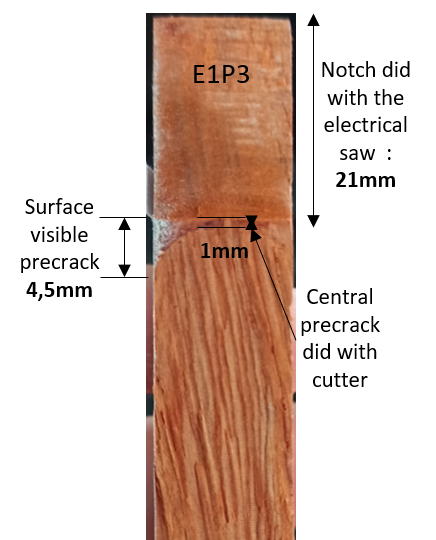
\includegraphics[scale=0.8]{Figures/Precrack}
	\decoRule
	\caption[Collapsed specimen]{Collapsed E1P3 specimen allowing to observe the real precrack length}
	\label{fig:Precrack}
\end{figure}

\begin{table}[h]
	\centering
	\begin{tabular}{c c }
		\multicolumn{1}{l}{} & \multicolumn{1}{l}{Used initial Crack length} \\
		\multicolumn{1}{c}{\cellcolor[HTML]{F8CBAD}E1O1} & 24,975   mm \\
		\multicolumn{1}{c}{\cellcolor[HTML]{F8CBAD}E1O2} & 24,25 mm \\
		\multicolumn{1}{c}{\cellcolor[HTML]{F8CBAD}E1O3} & 24,5 mm \\
		\multicolumn{1}{c}{\cellcolor[HTML]{C65911}E1P1} & 23,25 mm \\ 
		\cellcolor[HTML]{C65911}E1P2 & 23,4 mm \\ 
		\cellcolor[HTML]{C65911}E1P3 & 23,5 mm \\ 
		\multicolumn{1}{c}{\cellcolor[HTML]{BF8F00}E1I1} & 24,975 mm \\ 
		\multicolumn{1}{c}{\cellcolor[HTML]{F8CBAD}E2O1} & 26,475 mm \\ 
		\multicolumn{1}{c}{\cellcolor[HTML]{F8CBAD}E2O2} & 27,975 mm \\ 
		\multicolumn{1}{c}{\cellcolor[HTML]{F8CBAD}E2O3} & 29 mm \\ 
		\multicolumn{1}{c}{\cellcolor[HTML]{C65911}E2P1} & 27,4 mm \\ 
		\multicolumn{1}{c}{\cellcolor[HTML]{C65911}E2P2} & 27,9 mm \\ 
		\multicolumn{1}{c}{\cellcolor[HTML]{C65911}E2P3} & 27,5 mm \\ 
		\multicolumn{1}{c}{\cellcolor[HTML]{F8CBAD}E3O1} & 21,475 mm \\ 
		\multicolumn{1}{c}{\cellcolor[HTML]{F8CBAD}E3O2} & 22,75 mm \\ 
		\multicolumn{1}{c}{\cellcolor[HTML]{F8CBAD}E3O3} & 21,975 mm \\ 
		\multicolumn{1}{c}{\cellcolor[HTML]{C65911}E3P1} & 21,9 mm \\
		\multicolumn{1}{c}{\cellcolor[HTML]{C65911}E3P2} & 20,5 mm \\ 
		\multicolumn{1}{c}{\cellcolor[HTML]{C65911}E3P3} & 24,6 mm \\ 
		\multicolumn{1}{c}{\cellcolor[HTML]{F8CBAD}E4O1} & 23,975 mm \\ 
		\multicolumn{1}{c}{\cellcolor[HTML]{C65911}E4P1} & 23,25 mm \\ 
		\multicolumn{1}{c}{\cellcolor[HTML]{BF8F00}E4I1} & 23,975 mm \\ 
		\multicolumn{1}{c}{\cellcolor[HTML]{F8CBAD}E5O1} & 24 mm \\ 
		\multicolumn{1}{c}{\cellcolor[HTML]{C65911}E5P1} & 22,75 mm \\ 
		\multicolumn{1}{c}{\cellcolor[HTML]{BF8F00}E5I1} & 23,975 mm \\ 
		\multicolumn{1}{c}{\cellcolor[HTML]{C65911}Pbis} & 23,9 mm \\ 
		\multicolumn{1}{c}{\cellcolor[HTML]{C65911}Pter} & 23,25 mm \\ 
\end{tabular}
\caption{Precrack dimensions}
\label{tab:Tab11}
\end{table}
These values were obtained by the comparison of the surface precrack measured first and the look to the real precrack on \ref{fig:Precrack}. The equation used is shown in \ref{eq:precrack determination} :
\begin{equation}
	\centering
	\begin{array}{l}
		a_{0}= l_{notch} + \frac{l_{surfacic}+l_{interior}}{2}
		\\
		\\
		\left\{
		\begin{array}{llll}
			a_{0}: & $initial crack length$ & \si{\milli\meter} \\
			l_{notch}: & $notch length$ & \si{\milli\meter} \\
			l_{surfacic}: & $surfacic precrack measured$ & \si{\milli\meter} \\ 
			l_{interior}: & $real interior precrack measured$ & \si{\milli\meter} \\
		\end{array}
		\right.
	\end{array}
	\label{eq:precrack determination}
\end{equation} 
For some of the specimens, the crack was not done until the entire collapse. Then an approximation was made, using the average of the difference between the initial crack length measured and the one using \ref{eq:precrack determination} to have a more precise value. The average was made for each specie. Indeed, the average of this difference for Okoume specimen is around 1.525\si{\milli\meter} while the one for Padouck is 1.6\si{\milli\meter}. So this value was subtracted from the first measure, in order to take count of the non-uniform precrack.
All the specimens were weighed again, due to the material taken away by the creation of the notch.
%----------------------------------------------------------------------------------------
%	SUBSECTION 2
%----------------------------------------------------------------------------------------

\subsection{Moisture Content determination}

The literature review as shown some ways to determine the MC in specimens. The best way is to put specimens in a climatic room and wait until specimens have reached the expected MC thank to given climatic conditions input in the climatic room controller. Then a moisture meter can give instantly the MC into each sample. 

Without all this equipments, the formula \ref{eq:Moisture content depending on weight} is used. It means that many weight measurements must be done. 

So the 30 specimens bring from Polytech laboratory was weighed as soon as the sanitary condition (Covid pandemic) allows to do it. The scale used to weight the specimen was really precise, it is the GR-200 which is a Semi-Micro Analytical Balances. This precision is also made by the subtraction of air in the glass box, allowing a precision with the thousandths gram as visible on \ref{fig:Fig9}. Its capacity can not reach 210g which does not affect the measures with a max weight of the denser wood, the Padouck, around 70.5g and a minimum weight of Okoume specimens with a weight of 36g
\begin{figure}[th]
	\centering
	\includegraphics[scale=0.05,angle=-90]{Figures/Balance_Test}
	\decoRule
	\caption[GR-200 Scale]{GR-200 Scale weighing an Okoume specimen}
	\label{fig:Fig9}
\end{figure}

After this analyze, weight values were inputted in an Excel file. A resume is presented below in \ref{tab:Tab1} but the entire one is \ref{tab:Tab3}

\begin{table}[h]
\centering
\begin{tabular}{c r}
	\hline
	\cellcolor[rgb]{ .973,  .796,  .678}
	okoume average weight &
	\cellcolor[rgb]{ 1,  1,  1}
	40,55 g \\
	\cellcolor[rgb]{ .776,  .349,  .067}
	padouck average weight &
	\cellcolor[rgb]{ 1,  1,  1}
	66,29 g \\
	\cellcolor[rgb]{ .749,  .561,  0}
	iroko average weight &
	\cellcolor[rgb]{ 1,  1,  1}
	54,33 g \\
	\hline
\end{tabular}
\caption[specimens average weight]{specimens average weight depending on the species}
\label{tab:Tab1}
\end{table}
The next step was to dry them, in order to obtain the $M_{0}$ parameter, essential to approximate the MC. A drying process was done on all the specimens during 24h at 103\textcelsius. The scale was not the same and some specimens were weighed again before the drying process to obtain an uncertainty. The uncertainty was applied on every specimen and written in the Excel file. The purpose was to determine the potential difference of the weight between the specimen weight at the faculty and the one given a less precise scale. Then the drying experiment gives the $M_{0}$ weight of the samples. $M_{0}$ as explained is the dried weight of a sample in gram. It is used to calculate the moisture content in the sample. So, a new column was filled in the table \label{tab:Tab3} with the ambient moisture content. All the results are shown below, linked to the formula \ref{eq:Moisture content depending on weight}, given in previous chapters. The inaccuracy of the drying process, due to the scale change and also the time before weighting, the dried specimen do not allow to have the true MC rate in specimens. So all the specimens were dried and weight again, after being tested, thanks to the helpful Department of Civil Engineer of the FCT faculty. 

The average moisture content is around 9.20\% for Okoume specimens and 6.10\% for Padouck specimens. There are only three specimens of Iroko, which does not allow an efficient average, but it is around 7,5\% MC. It is important to notice that the specimen were dried and wait almost 24 hours before being weighted. That involves potential mistakes in the moisture content values calculated on the dried weight. But after another drying process, it appears that a delta exists and the average MC is more around 10.92\% for Okoume specimens, 8.05\% for Padouck and 9.03\% for Iroko specimens.

Specimens were weighed two times, to find the real difference between the scale from the laboratory and those from the drying process. A difference around 0.6g was found. Finally, specimens were put into water as it is visible on \ref{fig:Fig13}
\begin{figure}[h]
	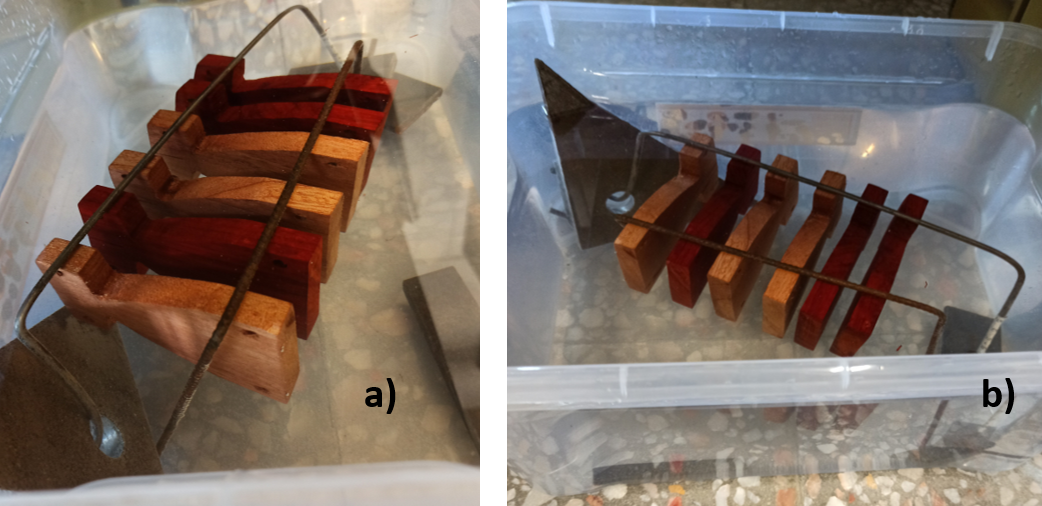
\includegraphics[width=\textwidth]{Figures/WaterSpecimens}
	\caption[Specimen moisture content increase]{Specimen moisture content increase experimental process.}
	\label{fig:Fig13}
\end{figure}

The system was designed in order to prevent the specimens from rising to the surface by flotation. But also, to minimize the specimen surface in contact with the system. Indeed, it allows to maximize the MC rise which take less time to reach the desired MC levels. This fact was verified when all the specimens (from E2 and E3 experiment) were put together into water. Of course, the system was not designed for 12 specimens, and the specimens were really closed. It involves a slower increase of the MC.

After 80.62h as presented in \ref{tab:MC_decrease}, specimens were weighed again. Thanks to these weights, it was possible to plot a shape about, how the MC decreases, and how the weight evolve compared to time. A quick look to the decrease of MC into Okoume specimens show that until 20\% MC, every hour almost 1\% MC is loose. From this value until the ambient MC, the MC decrease process becomes slower as it is shown on \ref{fig:Fig15_b}, with decreasment less than 0.4\% every hour.

Thanks to E3 daily weight, it appears that both species, Okoume and Padouck, earn a constant MC. The difference is the value of this constant increasing. Okoume specimens earn approximately 5\% MC each day, while Padouck ones earn around 2\% MC.

After the first serie of weight, some values were determined.
The purpose is to obtain specimen at a normal temperature, but with a maximum moisture content around 30\%. So by weighting every hour specimens submersed for days, the MC evolution of samples can be expected. One table was created for each specimen as the \ref{tab:MC_decrease} one.

\begin{table}[]
	\centering
	\begin{tabular}{llll}
		\cline{1-2}
		\multicolumn{1}{c}{\cellcolor[HTML]{F8CBAD}E2O1} & \multicolumn{1}{c}{\cellcolor[HTML]{F8CBAD}34,219} & 9,83\% &  \\ \cline{1-2}
		&  &  &  \\ 
		\multicolumn{1}{c}{time} & \multicolumn{1}{c}{Wet Weight} & \multicolumn{1}{c}{MC} & \multicolumn{1}{c}{MC decreasment O1} \\ 
		\multicolumn{1}{l}{\cellcolor[HTML]{A5A5A5}09:13:00} & \multicolumn{1}{l}{67 g} & \multicolumn{1}{l}{95,79765627   \%} &  \\ \cline{1-3}
		\multicolumn{1}{l}{10:22:00} & \multicolumn{1}{l}{66 g} & \multicolumn{1}{l}{92,87530319   \%} &  \\ \cline{1-3}
		\multicolumn{1}{l}{11:22:00} & \multicolumn{1}{l}{65 g} & \multicolumn{1}{l}{89,95295012   \%} &  \\ 
		\multicolumn{1}{l}{12:22:00} & \multicolumn{1}{l}{64 g} & \multicolumn{1}{l}{87,03059704   \%} & \multicolumn{1}{l}{\cellcolor[HTML]{A5A5A5}Day change} \\ 
		\multicolumn{1}{l}{13:22:00} & \multicolumn{1}{l}{63 g} & \multicolumn{1}{l}{84,10824396   \%} & \multicolumn{1}{l}{\cellcolor[HTML]{9BC2E6}Scale change} \\ 
		\multicolumn{1}{l}{14:22:00} & \multicolumn{1}{l}{60 g} & \multicolumn{1}{l}{75,34118472   \%} & \multicolumn{1}{l}{\cellcolor[HTML]{00B0F0}20\% MC reached} \\ 
		\multicolumn{1}{l}{15:22:00} & \multicolumn{1}{l}{60 g} & \multicolumn{1}{l}{75,34118472   \%} & \multicolumn{1}{l}{\cellcolor[HTML]{0070C0}30\% MC reached} \\ 
		\multicolumn{1}{l}{16:35:00} & \multicolumn{1}{l}{59 g} & \multicolumn{1}{l}{72,41883164   \%} & \multicolumn{1}{l}{\cellcolor[HTML]{FFC000}Normal MC reached} \\ 
		\multicolumn{1}{l}{17:43:00} & \multicolumn{1}{l}{59 g} & \multicolumn{1}{l}{72,41883164   \%} &  \\ 
		\multicolumn{1}{l}{18:26:00} & \multicolumn{1}{l}{59 g} & \multicolumn{1}{l}{72,41883164   \%} &  \\ 
		\multicolumn{1}{l}{19:30:00} & \multicolumn{1}{l}{58 g} & \multicolumn{1}{l}{69,49647856   \%} &  \\ 
		\multicolumn{1}{l}{20:37:00} & \multicolumn{1}{l}{56 g} & \multicolumn{1}{l}{63,65177241   \%} &  \\ 
		\multicolumn{1}{l}{21:50:00} & \multicolumn{1}{l}{56 g} & \multicolumn{1}{l}{63,65177241   \%} &  \\ 
		\multicolumn{1}{l}{22:22:00} & \multicolumn{1}{l}{56 g} & \multicolumn{1}{l}{63,65177241   \%} &  \\ 
		\multicolumn{1}{l}{23:05:00} & \multicolumn{1}{l}{55 g} & \multicolumn{1}{l}{60,72941933   \%} &  \\ 
		\multicolumn{1}{l}{00:09:00} & \multicolumn{1}{l}{53 g} & \multicolumn{1}{l}{54,88471317   \%} &  \\ 
		\multicolumn{1}{l}{01:24:00} & \multicolumn{1}{l}{53 g} & \multicolumn{1}{l}{54,88471317   \%} &  \\ 
		\multicolumn{1}{l}{\cellcolor[HTML]{A5A5A5}07:45:00} & \multicolumn{1}{l}{50 g} & \multicolumn{1}{l}{46,11765393   \%} &  \\ 		\multicolumn{1}{l}{09:10:00} & \multicolumn{1}{l}{49 g} & \multicolumn{1}{l}{43,19530086   \%} &  \\ 
		\multicolumn{1}{l}{09:48:00} & \multicolumn{1}{l}{\cellcolor[HTML]{9BC2E6}51,535 g} & \multicolumn{1}{l}{50,60346591   \%} &  \\ 
		\multicolumn{1}{l}{10:49:00} & \multicolumn{1}{l}{51,114 g} & \multicolumn{1}{l}{49,37315526   \%} & \multicolumn{1}{l}{1,230310646 \%} \\ 
		\multicolumn{1}{l}{11:29:00} & \multicolumn{1}{l}{50,737 g} & \multicolumn{1}{l}{48,27142815   \%} & \multicolumn{1}{l}{1,101727111 \%} \\ 
		\multicolumn{1}{l}{12:30:00} & \multicolumn{1}{l}{50,207 g} & \multicolumn{1}{l}{46,72258102   \%} & \multicolumn{1}{l}{1,548847132 \%} \\ 
		\multicolumn{1}{l}{13:45:00} & \multicolumn{1}{l}{49,624 g} & \multicolumn{1}{l}{45,01884918   \%} & \multicolumn{1}{l}{1,703731845 \%} \\ 
		\multicolumn{1}{l}{14:45:00} & \multicolumn{1}{l}{49,225 g} & \multicolumn{1}{l}{43,8528303   \%} & \multicolumn{1}{l}{1,166018878 \%} \\ 
		\multicolumn{1}{l}{15:40:00} & \multicolumn{1}{l}{48,811 g} & \multicolumn{1}{l}{42,64297612   \%} & \multicolumn{1}{l}{1,209854175 \%} \\ 
		\multicolumn{1}{l}{16:36:00} & \multicolumn{1}{l}{48,368 g} & \multicolumn{1}{l}{41,34837371   \%} & \multicolumn{1}{l}{1,294602414 \%} \\ 
		\multicolumn{1}{l}{\cellcolor[HTML]{A5A5A5}09:39:00} & \multicolumn{1}{l}{44,397 g} & \multicolumn{1}{l}{29,74370963   \%} &  \\ 
		\multicolumn{1}{l}{10:34:00} & \multicolumn{1}{l}{43,994 g} & \multicolumn{1}{l}{28,56600134   \%} & \multicolumn{1}{l}{1,177708291 \%} \\ 
		\multicolumn{1}{l}{11:34:00} & \multicolumn{1}{l}{43,612 g} & \multicolumn{1}{l}{27,44966247   \%} & \multicolumn{1}{l}{1,116338876 \%} \\ 
		\multicolumn{1}{l}{13:09:00} & \multicolumn{1}{l}{43,048 g} & \multicolumn{1}{l}{25,80145533   \%} & \multicolumn{1}{l}{1,648207136 \%} \\ 
		\multicolumn{1}{l}{14:26:00} & \multicolumn{1}{l}{42,624 g} & \multicolumn{1}{l}{24,56237763   \%} & \multicolumn{1}{l}{1,239077705 \%} \\ 
		\multicolumn{1}{l}{15:38:00} & \multicolumn{1}{l}{42,279 g} & \multicolumn{1}{l}{23,55416581   \%} & \multicolumn{1}{l}{1,008211812 \%} \\ 
		\multicolumn{1}{l}{16:39:00} & \multicolumn{1}{l}{41,979 g} & \multicolumn{1}{l}{22,67745989   \%} & \multicolumn{1}{l}{0,876705924 \%} \\ 
		\multicolumn{1}{l}{18:44:00} & \multicolumn{1}{l}{41,444 g} & \multicolumn{1}{l}{21,11400099   \%} &  \\ 
		\multicolumn{1}{l}{19:34:00} & \multicolumn{1}{l}{41,323 g} & \multicolumn{1}{l}{20,76039627   \%} & \multicolumn{1}{l}{0,353604723 \%} \\ 
		\multicolumn{1}{l}{\cellcolor[HTML]{A5A5A5}09:22:00} & \multicolumn{1}{l}{39,327 g} & \multicolumn{1}{l}{14,92737953   \%} &  \\ 
		\multicolumn{1}{l}{10:35:00} & \multicolumn{1}{l}{39,196 g} & \multicolumn{1}{l}{14,54455127   \%} & \multicolumn{1}{l}{0,382828253 \%} \\ 
		\multicolumn{1}{l}{11:32:00} & \multicolumn{1}{l}{39,098 g} & \multicolumn{1}{l}{14,25816067   \%} & \multicolumn{1}{l}{0,286390602 \%} \\ 
		\multicolumn{1}{l}{13:12:00} & \multicolumn{1}{l}{38,931 g} & \multicolumn{1}{l}{13,77012771   \%} & \multicolumn{1}{l}{0,488032964 \%} \\ 
		\multicolumn{1}{l}{14:12:00} & \multicolumn{1}{l}{38,833 g} & \multicolumn{1}{l}{13,48373711   \%} & \multicolumn{1}{l}{0,286390602 \%} \\ 
		\multicolumn{1}{l}{15:14:00} & \multicolumn{1}{l}{38,768 g} & \multicolumn{1}{l}{13,29378416   \%} & \multicolumn{1}{l}{0,18995295 \%} \\ 
		\multicolumn{1}{l}{16:06:00} & \multicolumn{1}{l}{38,702 g} & \multicolumn{1}{l}{13,10090885   \%} & \multicolumn{1}{l}{0,192875303 \%} \\ 
		\multicolumn{1}{l}{17:00:00} & \multicolumn{1}{l}{38,652 g} & \multicolumn{1}{l}{12,9547912   \%} & \multicolumn{1}{l}{0,146117654 \%} \\ 
	\end{tabular}
	\caption{Moisture Content and weight decrease depending on time with the E2O1 specimen example}
	\label{tab:MC_decrease}
\end{table}

It is important to notice that the scale change, from a normal one to a really precise one, did not allow to obtain a good curve shape during the first day of weight, as visible on \ref{fig:Fig15_a} and \ref{fig:Fig15_c}. Indeed, \ref{tab:MC_decrease} first values have a gram precision and the scale had a strange behavior. This is also why, the MC decrease on \ref{fig:Fig15_b} and \ref{fig:Fig15_d} was not calculated during these first days. 
\begin{figure}[th]
	\centering
	\begin{subfigure}{0.48\linewidth}
		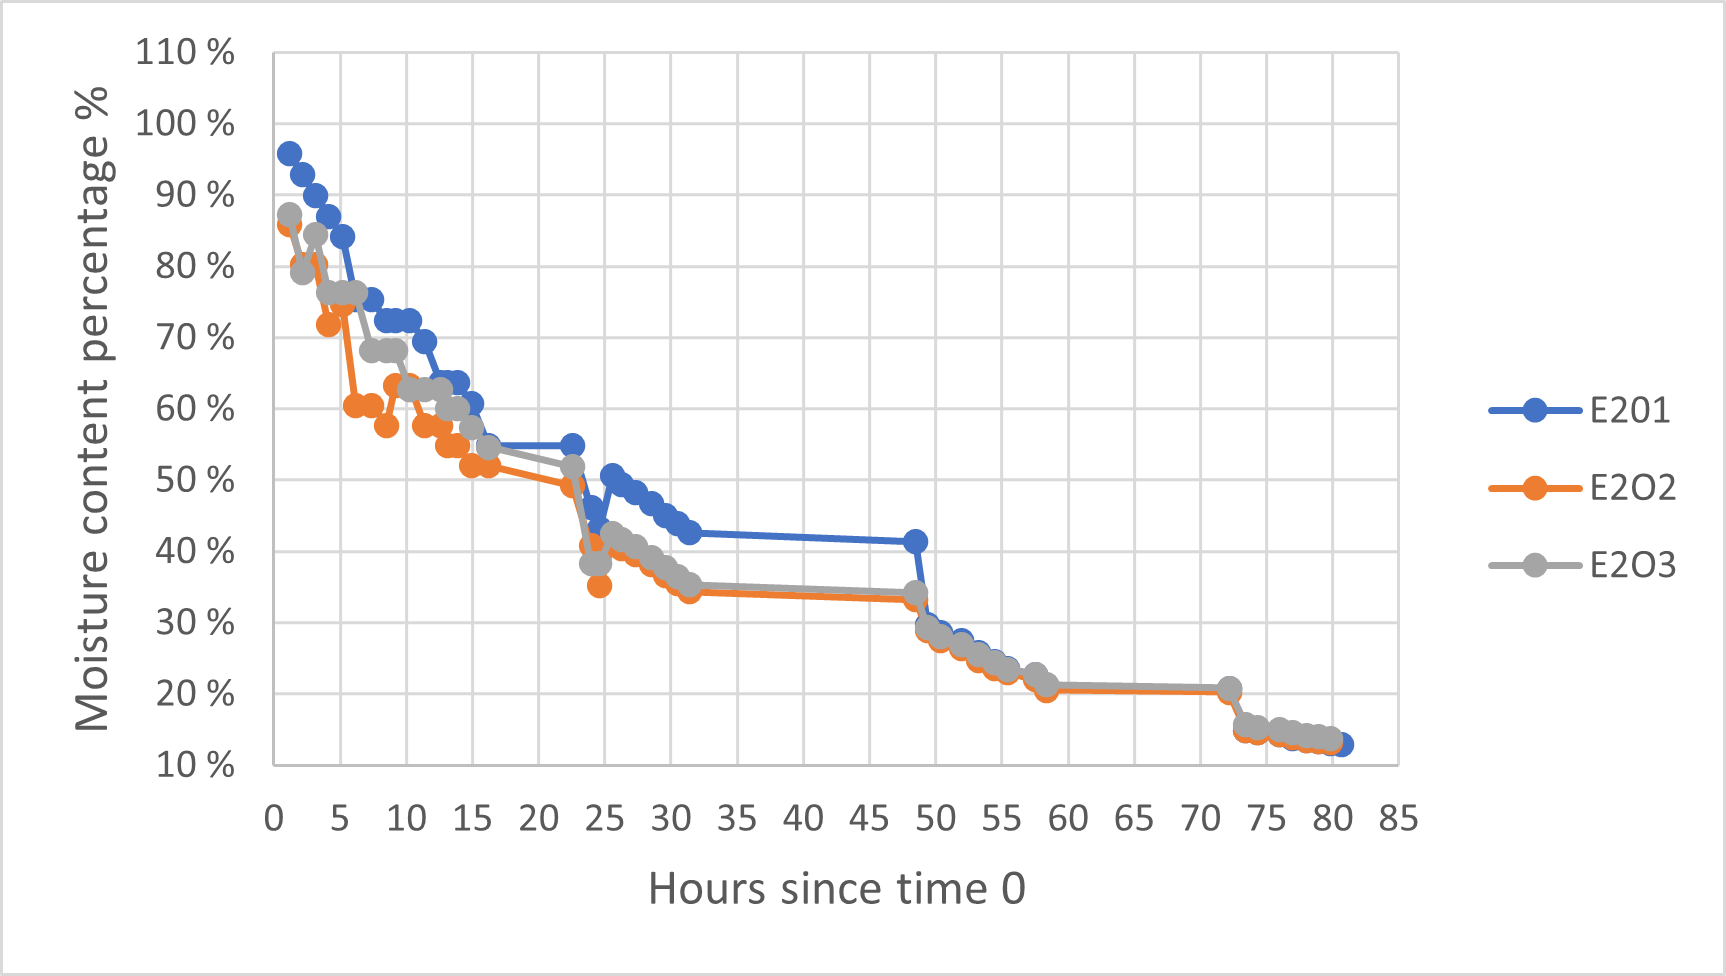
\includegraphics[width=\textwidth]{Figures/Okoume_MCdecreas}
		\caption[Okoume MC decrease depending on time.]{Plot of 3 Okoume specimens MC decrease depending on time.}
		\label{fig:Fig15_a}
	\end{subfigure}
	\hfill
	\begin{subfigure}{0.48\linewidth}
		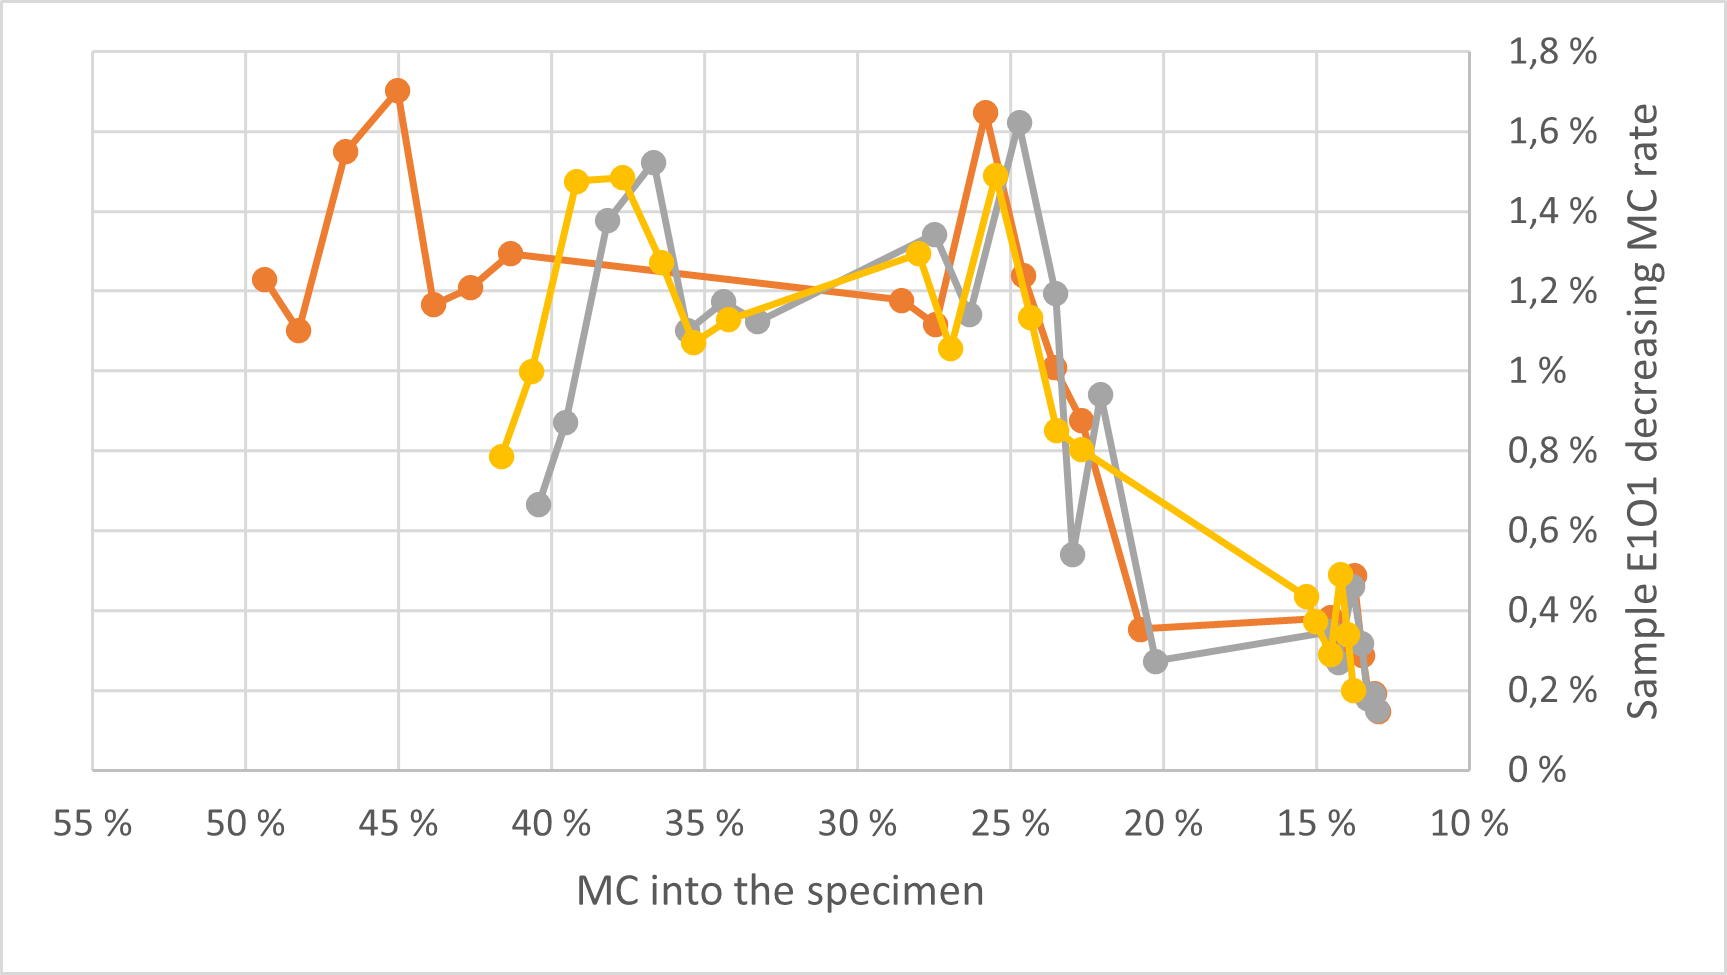
\includegraphics[width=\textwidth]{Figures/Okoume_MCevol}
		\caption[MC decreassement depending on MC for 3 Okoume samples]{Plot of 3 Okoume specimens MC decreassement depending on MC}
		\label{fig:Fig15_b}
	\end{subfigure}
		\hfill
	\begin{subfigure}{0.48\linewidth}
		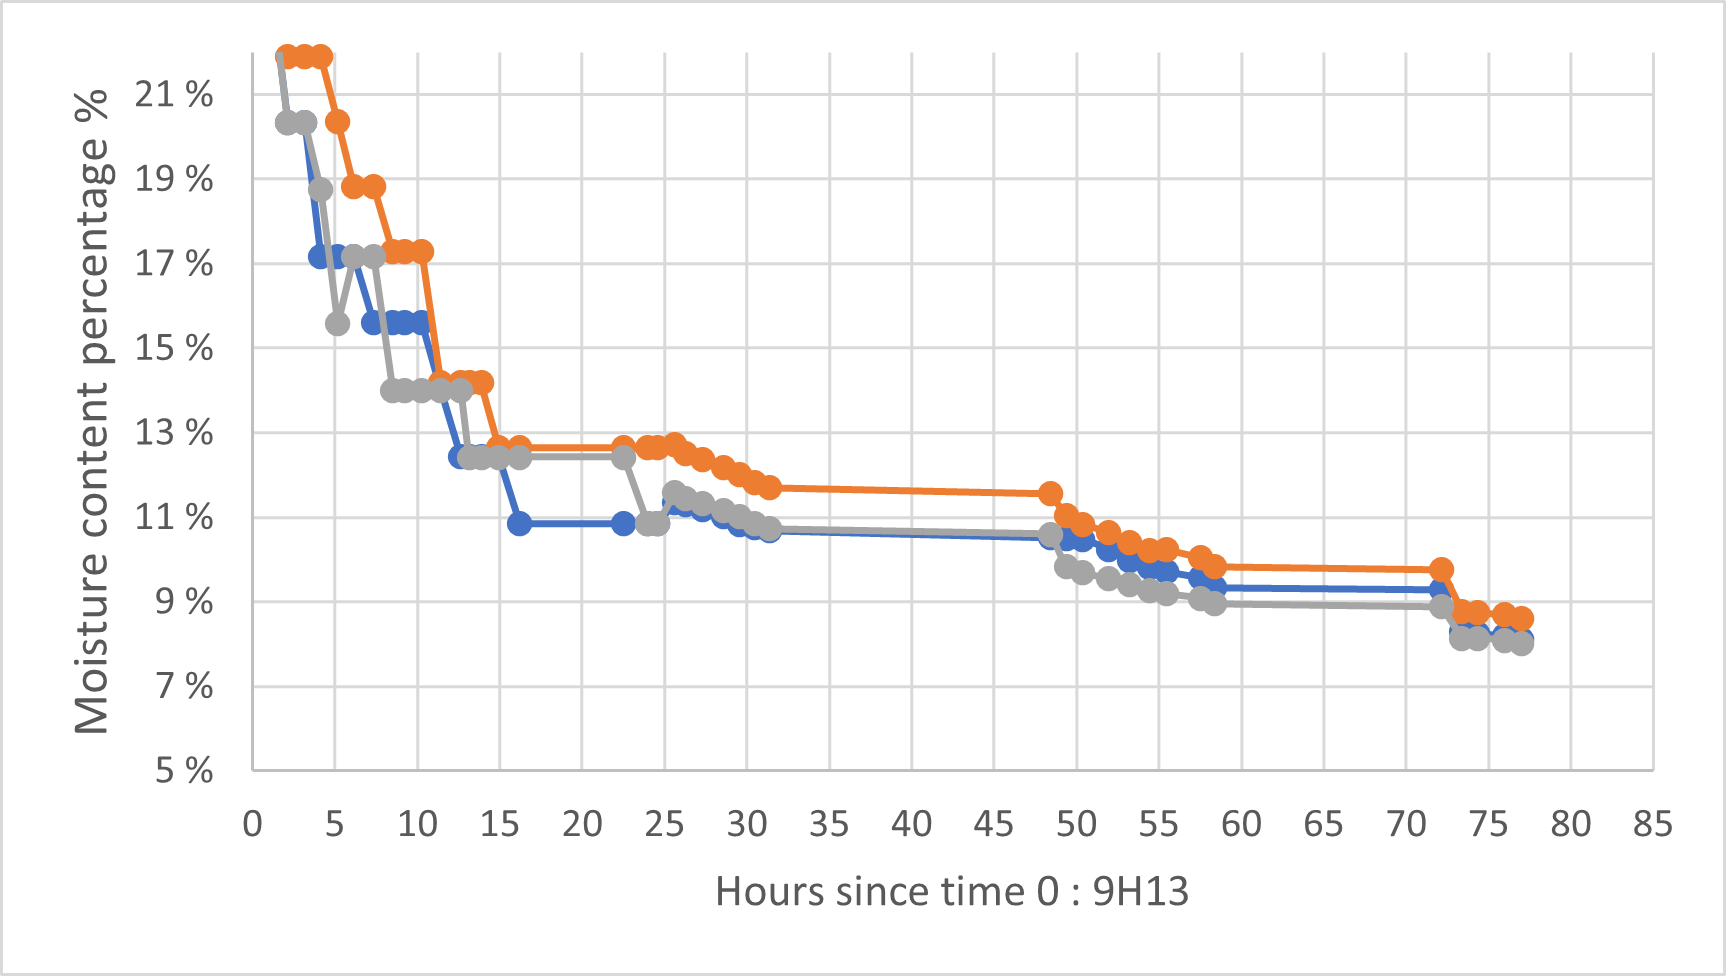
\includegraphics[width=\textwidth]{Figures/Padouck_MCdecreas}
		\caption[Padouck MC decrease depending on time.]{Plot of 3 Padouck specimens MC decrease depending on time.}
		\label{fig:Fig15_c}
	\end{subfigure}
		\hfill
	\begin{subfigure}{0.48\linewidth}
		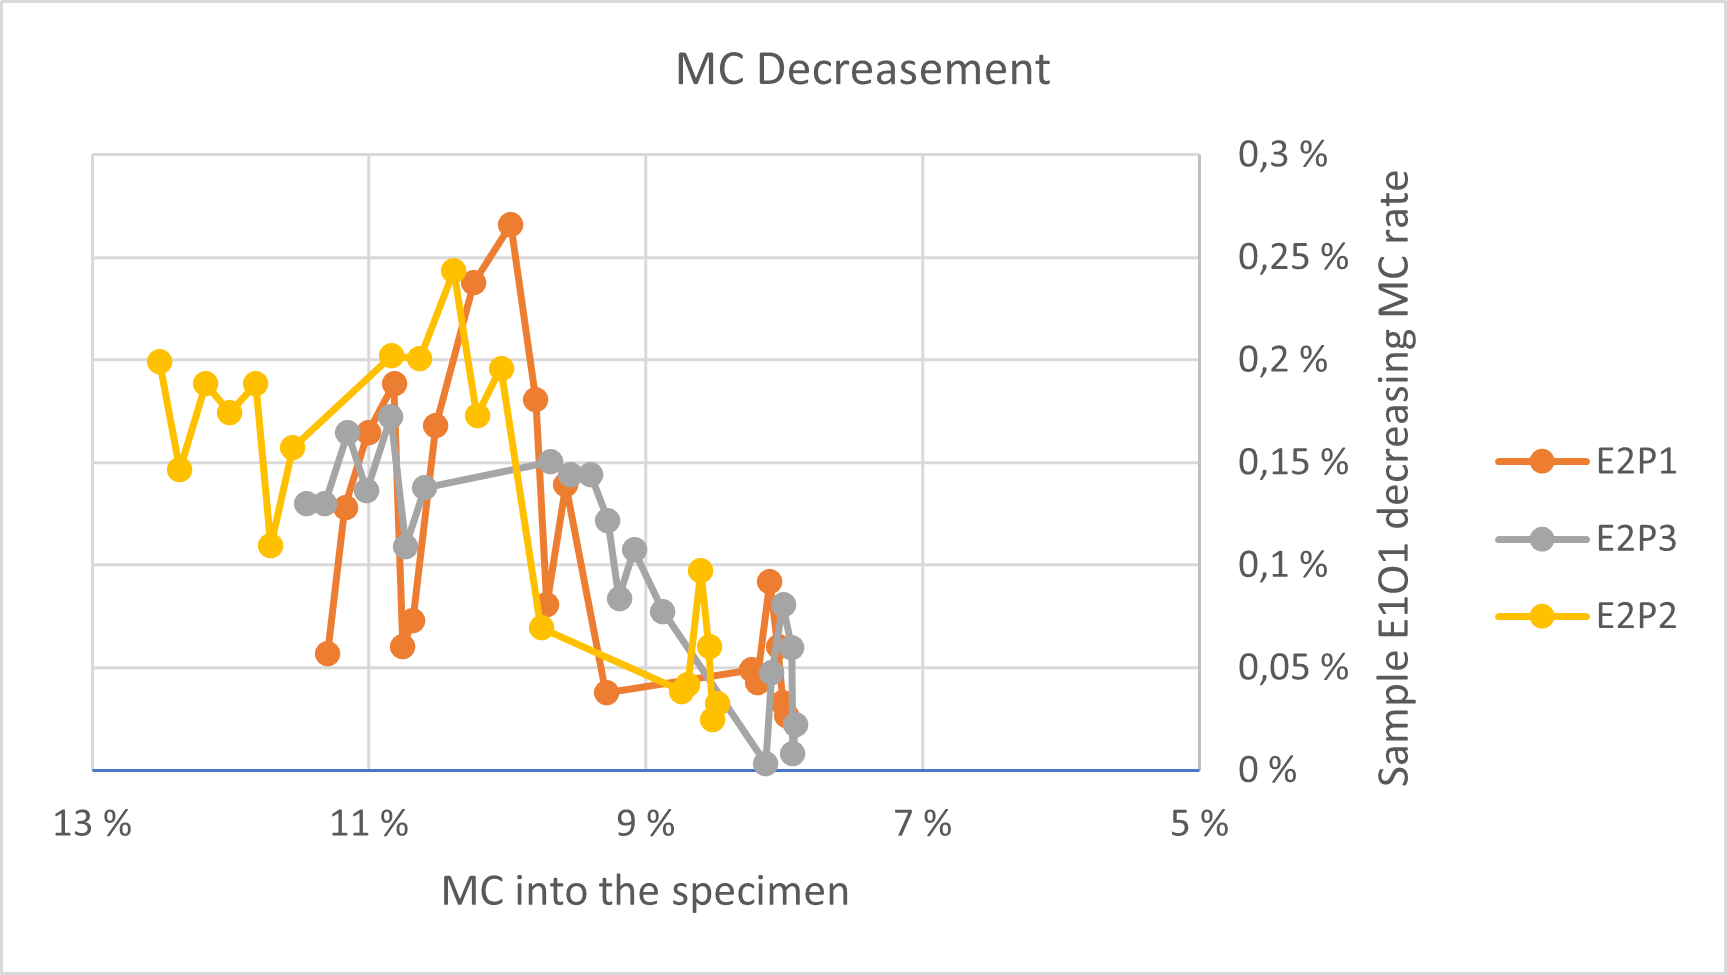
\includegraphics[width=\textwidth]{Figures/Padouck_MCevol}
		\caption[MC decreassement depending on MC for 3 Padouck samples]{Plot of 3 Padouck specimens MC decreassement depending on MC}
		\label{fig:Fig15_d}
	\end{subfigure}
	\caption{MC evolution of specimens}
	\label{fig:Fig15}
	
\end{figure}

Unfortunately, the two important steps, at 20\% and 30\% were reached at a time when the measurement were not done every hour as it is visible on \ref{fig:Fig15_a} or \ref{fig:Fig15_c}. But it allows to have the shape of the curve, showing how the MC decreases depending on time. Thanks to these curves, it was possible to predict, regarding the hours at which the specimens were put off the water, when they must be tested to have the approximate MC expected.

But wood is a living material with a really particular behavior. Looking to this previous parameters, visible in \ref{fig:Fig15_a} and \ref{fig:Fig15_b} an approximation was made. By putting out of the water the specimens at a given hour, they will be tested at a given other. By processing this way, a lot of the experiments were sceduled for 53h after putting them off the water. But in 7 hours Okoume specimen loose around 20\% of MC and Padouck around 7\%. Which is following the previous curve, but for Padouck specimen it was quicker than expected.

%----------------------------------------------------------------------------------------
%	SUBSECTION 3
%----------------------------------------------------------------------------------------

\subsection{Chosen experiments}

Due to the delay and the material made available, some tests could not be done. It was chosen to only study the evolution of energy release rate by the variation of MC. To have more data and create a smoother curve of results, the specimens expected to be tested at different temperature were put into water to increase their MC and have values at a different MC than the average of 20\% and 30\%. It must be noted that, at the contrary of samples scheduled to be tested at different MC, E4 and E5 specimens were put off the water during the morning and tested during the afternoon. They were more wet, so a different behavior was expected.In the same time, Silver Fir specimens were sent from France, to be tested and compared as intended first. Unfortunately, they were waited too long and it was impossible to put them into water in order to obtain results as the same MC as the others species. Therefore, they never arrived and this work is focused on Padouck and Okoume species tested at room humidity, and at 20\%, 30\% MC.

%%%%%%%%%%%%%%%%%%%%%%%%%%%%%%%%%%%%%%%%%%%%%%%%%%%%%%%%%%%
%%%%%%%%%%%%%%%%%%%%%%%%%%%%%%%%%%%%%%%%%%%%%%%%%%%%%%%%%%%


%
%\section{Mode I fracture loading test using the MMCG specimen: data reduction}
%
%\section{Python Code to analysed datas}
%
%\begin{lstlisting}[language=Python]
%import numpy as np
%
%def incmatrix(genl1,genl2):
%    m = len(genl1)
%    n = len(genl2)
%    M = None #to become the incidence matrix
%    VT = np.zeros((n*m,1), int)  #dummy variable
%
%    #compute the bitwise xor matrix
%    M1 = bitxormatrix(genl1)
%    M2 = np.triu(bitxormatrix(genl2),1)
%
%    for i in range(m-1):
%        for j in range(i+1, m):
%            [r,c] = np.where(M2 == M1[i,j])
%            for k in range(len(r)):
%                VT[(i)*n + r[k]] = 1;
%                VT[(i)*n + c[k]] = 1;
%                VT[(j)*n + r[k]] = 1;
%                VT[(j)*n + c[k]] = 1;
%
%                if M is None:
%                    M = np.copy(VT)
%                else:
%                    M = np.concatenate((M, VT), 1)
%
%                VT = np.zeros((n*m,1), int)
%
%    return M
%\end{lstlisting}
%
%\lstinputlisting[language=Python, firstline=180, lastline=202]{Figures/pyMMCG.py}
%

%
%Then, 
%
% :::::::::::::::::::::::::::::::::::::::::::::::::::::
%
%
%
